%
\documentclass{article}
\newcommand{\assgnnum}{4}
\newcommand{\duedate}{January 28}

\usepackage{amsmath}
\usepackage{fullpage}
\usepackage{amssymb}
%\usepackage{bbm}
\usepackage{fancyhdr}
%\usepackage{paralist}
\usepackage{graphicx}
\usepackage{caption}
\usepackage{subcaption}
\usepackage[pdftex,colorlinks=true, urlcolor = blue]{hyperref}
\usepackage{../../arbenson-math}


\oddsidemargin 0in \evensidemargin 0in
\topmargin -0.5in \headheight 0.25in \headsep 0.25in
\textwidth 6.5in \textheight 9in
\parskip 6pt \parindent 0in \footskip 20pt

% set the header up
\fancyhead{}
\fancyhead[L]{CME193: Assignment \assgnnum}
\fancyhead[R]{Due: \duedate}
%%%%%%%%%%%%%%%%%%%%%%%%%%
\renewcommand\headrulewidth{0.4pt}
\setlength\headheight{15pt}

\newcommand{\p}{\ensuremath{\mathbf{P}}}
\renewcommand{\Pr}[1]{\ensuremath{\p \left \{ #1 \right \}}}
\newcommand{\nti}{\ensuremath{n \to \infty}}
\newcommand{\I}{\ensuremath{\operatorname{I}}}
\newcommand{\One}[1]{\ensuremath{\mathbbm{1}_{\left \{ #1 \right \}}}}
\newcommand{\E}{\ensuremath{\mathbf{E}}}
\newcommand{\Ex}[2][]{\ensuremath{\E_{#1} \left[ #2 \right]}}
\newcommand{\var}{\ensuremath{\operatorname{Var}}}
\newcommand{\cov}{\ensuremath{\operatorname{Cov}}}
\newcommand{\F}{\ensuremath{\mathcal{F}}}
\newcommand{\R}{\ensuremath{\mathbb{R}}}
\newcommand{\C}{\ensuremath{\mathbb{C}}}
\newcommand{\NormRV}[2]{\ensuremath{\operatorname{N}\left(#1, #2\right)}}
\newcommand{\BetaRV}[2]{\ensuremath{\operatorname{Beta}\left(#1, #2\right)}}
\newcommand{\argmax}{\operatornamewithlimits{argmax}}
\newcommand{\x}{\mathbf{x}}
\newcommand{\A}{\mathbf{A}}
\newcommand{\bb}{\mathbf{b}}

\newcounter{points}
\setcounter{points}{0}
\newcounter{bonuspoints}
\setcounter{bonuspoints}{0}

\newcommand\setpoints[1]{\addtocounter{points}{#1}(#1 points)}
\newcommand\setpoint{\addtocounter{points}{1}(1 point)}
\newcommand\setbonuspoints[1]{\addtocounter{bonuspoints}{#1}(#1 bonus points)}
\newcommand\setbonuspoint{\addtocounter{bonuspoints}{1}(1 bonus point)}


\newcommand{\eqD}{\ensuremath{\overset{\mathcal{D}}{=}}}

\setlength{\parindent}{0in}
\graphicspath{ {./figures/} }

\begin{document}

\pagestyle{fancy}
%\vspace*{15pt}

The auto-grader will run tests against your code, all of which must pass for you to pass the assignment. Remember: you must pass all assignments to pass the class. Do not use the function np.vectorize anywhere in this assignment.

\begin{enumerate}
\item \textbf{Profiling and Vectorization} \setpoints{15} \\
In this question we are going to use Python profiling tools to determine the efficiency of using NumPy's vectorization capabilities. To do so we will compute the first 100 powers (exclusive and starting from 0) of 2 in the following ways. Use the \texttt{main()} method in \texttt{prof.py} to investigate the amount of time it takes to run each of these methods 100,000 times.
\vspace{.1in}

To profile each of the statements you will create, use the \texttt{timeit} module. There are many ways to use this module (see
\url{ http://docs.python.org/2.7/library/timeit.html}) but you should only need to use the \texttt{timeit.timeit()} function which is implemented in the \texttt{main()} method. 

\begin{enumerate}
\item append  to an initially empty list sequentially in \texttt{empty\_list()}
\item create an list of zeros of size 100 and assign elements sequentially in \texttt{preallocated\_list()}
\item use a list comprehension in \texttt{lst\_comp()}
\item use the python map function in \texttt{map\_twos()}
\item use vectorization (NumPy) in  \texttt{twos\_numpy()}
\end{enumerate}

\item \textbf{SciPy Optimization} \setpoints{15}

The \texttt{scipy.optimize} module contains functions that perform numerical optimization. Use \newline
\texttt{scipy.optimize.fmin} to minimize the following function with starter code in \texttt{scipy\_opt.py} using the function \texttt{test\_opt()}. If your version of scipy does not have
\texttt{scipy.optimize.fmin}, use \texttt{scipy.optimize.fmin\_bfgs}.
$$f(x) = \frac{1}{2}x^TAx - b^Tx$$
When 
$A= \begin{pmatrix}
1 & 1\\
1 & 2
\end{pmatrix}$
and $b = \begin{pmatrix}
1 \\
1 \\
\end{pmatrix}$.
Verify that your solution $x^*$ is a solution to the system of linear equations defined by $A$ and $b$ by passing your solution $x^*$, $A$ and $b$ to \texttt{verify\_opt()}. That is, make sure $Ax^*=b$.

\newpage
\item \textbf{Kernel Density Estimate (KDE)} \setpoints{20}

Given a sample $x_1, x_2, \dots, x_n$ from an unknown distribution $f$ the kernel density estimate of $f$ at point $x$ with kernel $K_b$ is defined as 
$$\hat{f}(x;b) = \frac{1}{n}\sum_{i=1}^{n}K_b(x-x_i)$$
where the kernel must satisfy $\int_{-\infty}^{\infty}K(u)du = 1$ and $K(-u) = K(u).$ The parameter $b$ is known as the bandwidth and controls the width of the kernel used. There are many possible choices for kernels, and we will use the triangular kernel

$$K_{b}(z) = \frac{1}{b}(1 - |\frac{z}{b}|)\mathbb{*I}(|\frac{z}{b} |\leq 1)$$ 

\begin{figure}[h!!!]
        \centering
        \begin{subfigure}[b]{0.48\textwidth}
        \centering
        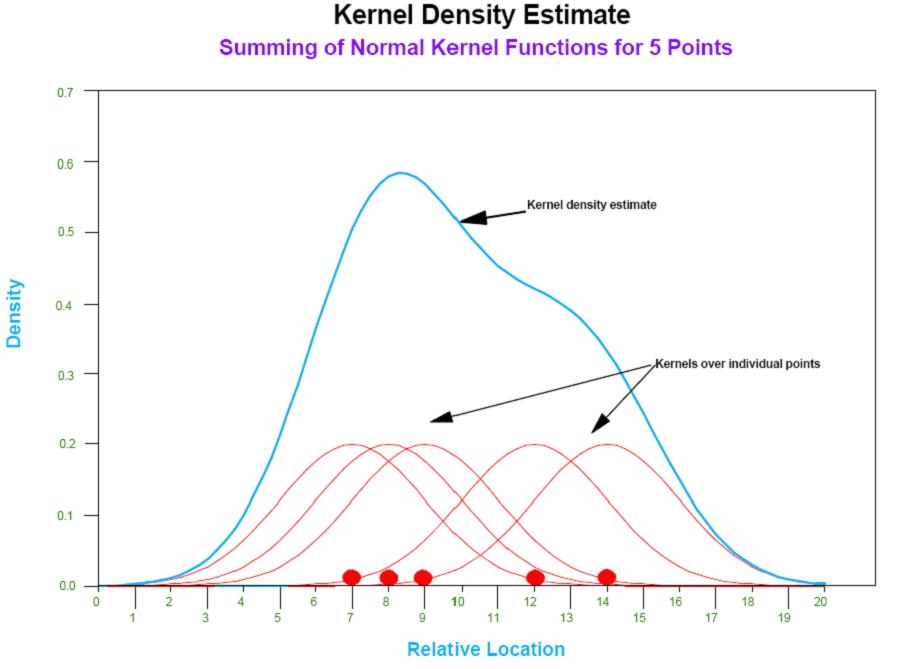
\includegraphics[height=1.9in, natwidth=410,natheight=442]{kde}
        \caption{Gaussian Kernel Density Estimate}
        \label{fig:gkde}
        \end{subfigure}
        \quad
        \centering
        \begin{subfigure}[b]{0.48\textwidth}
        \centering
        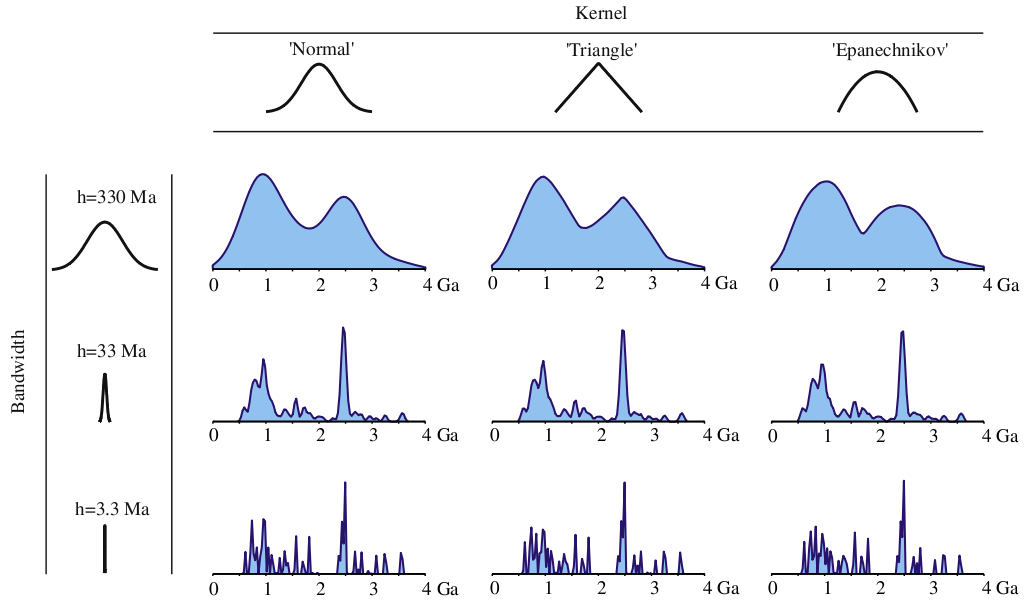
\includegraphics[height=1.9in, natwidth=410,natheight=442]{bw}
        \caption{Bandwiths and Kernels}
        \label{fig:bw}
        \end{subfigure}
\end{figure}

Write a ONE line python function without list comprehension or the keyword \texttt{for} that takes the three parameters below and returns $\hat{f}(x)$, the KDE evaluated at $x$.  Implement this in \texttt{kde.py}. 
\begin{enumerate}
\item \texttt{x} the point to evaluate the KDE
\item \texttt{data}  the sample of points from $f$  ; above denoted $x_1, x_2, \dots, x_n$ 
\item \texttt{bw} the bandwidth of the kernel
\end{enumerate}



\item \textbf{matplotlib} \setpoints{0}

It will be useful to have matplotlib installed for lecture 5. Please install \texttt{matplotlib} on your system and make sure the following lines produce a graph 
\begin{verbatim}
>>> import matplotlib.pyplot as plt
>>> plt.plot(np.arange(10))
>>> plt.show()
\end{verbatim}
\end{enumerate}
%\printpoints.
\end{document} 
